\chapter{Sample Chapter}\label{chap:Sample}
{\color{blue} Located in {\ttfamily Sample.tex}}\\





Sample chapter text goes here.  For complex documents you may want sub-folders for each chapter and associated figures. 



\begin{figure}[ht]
    \centering
    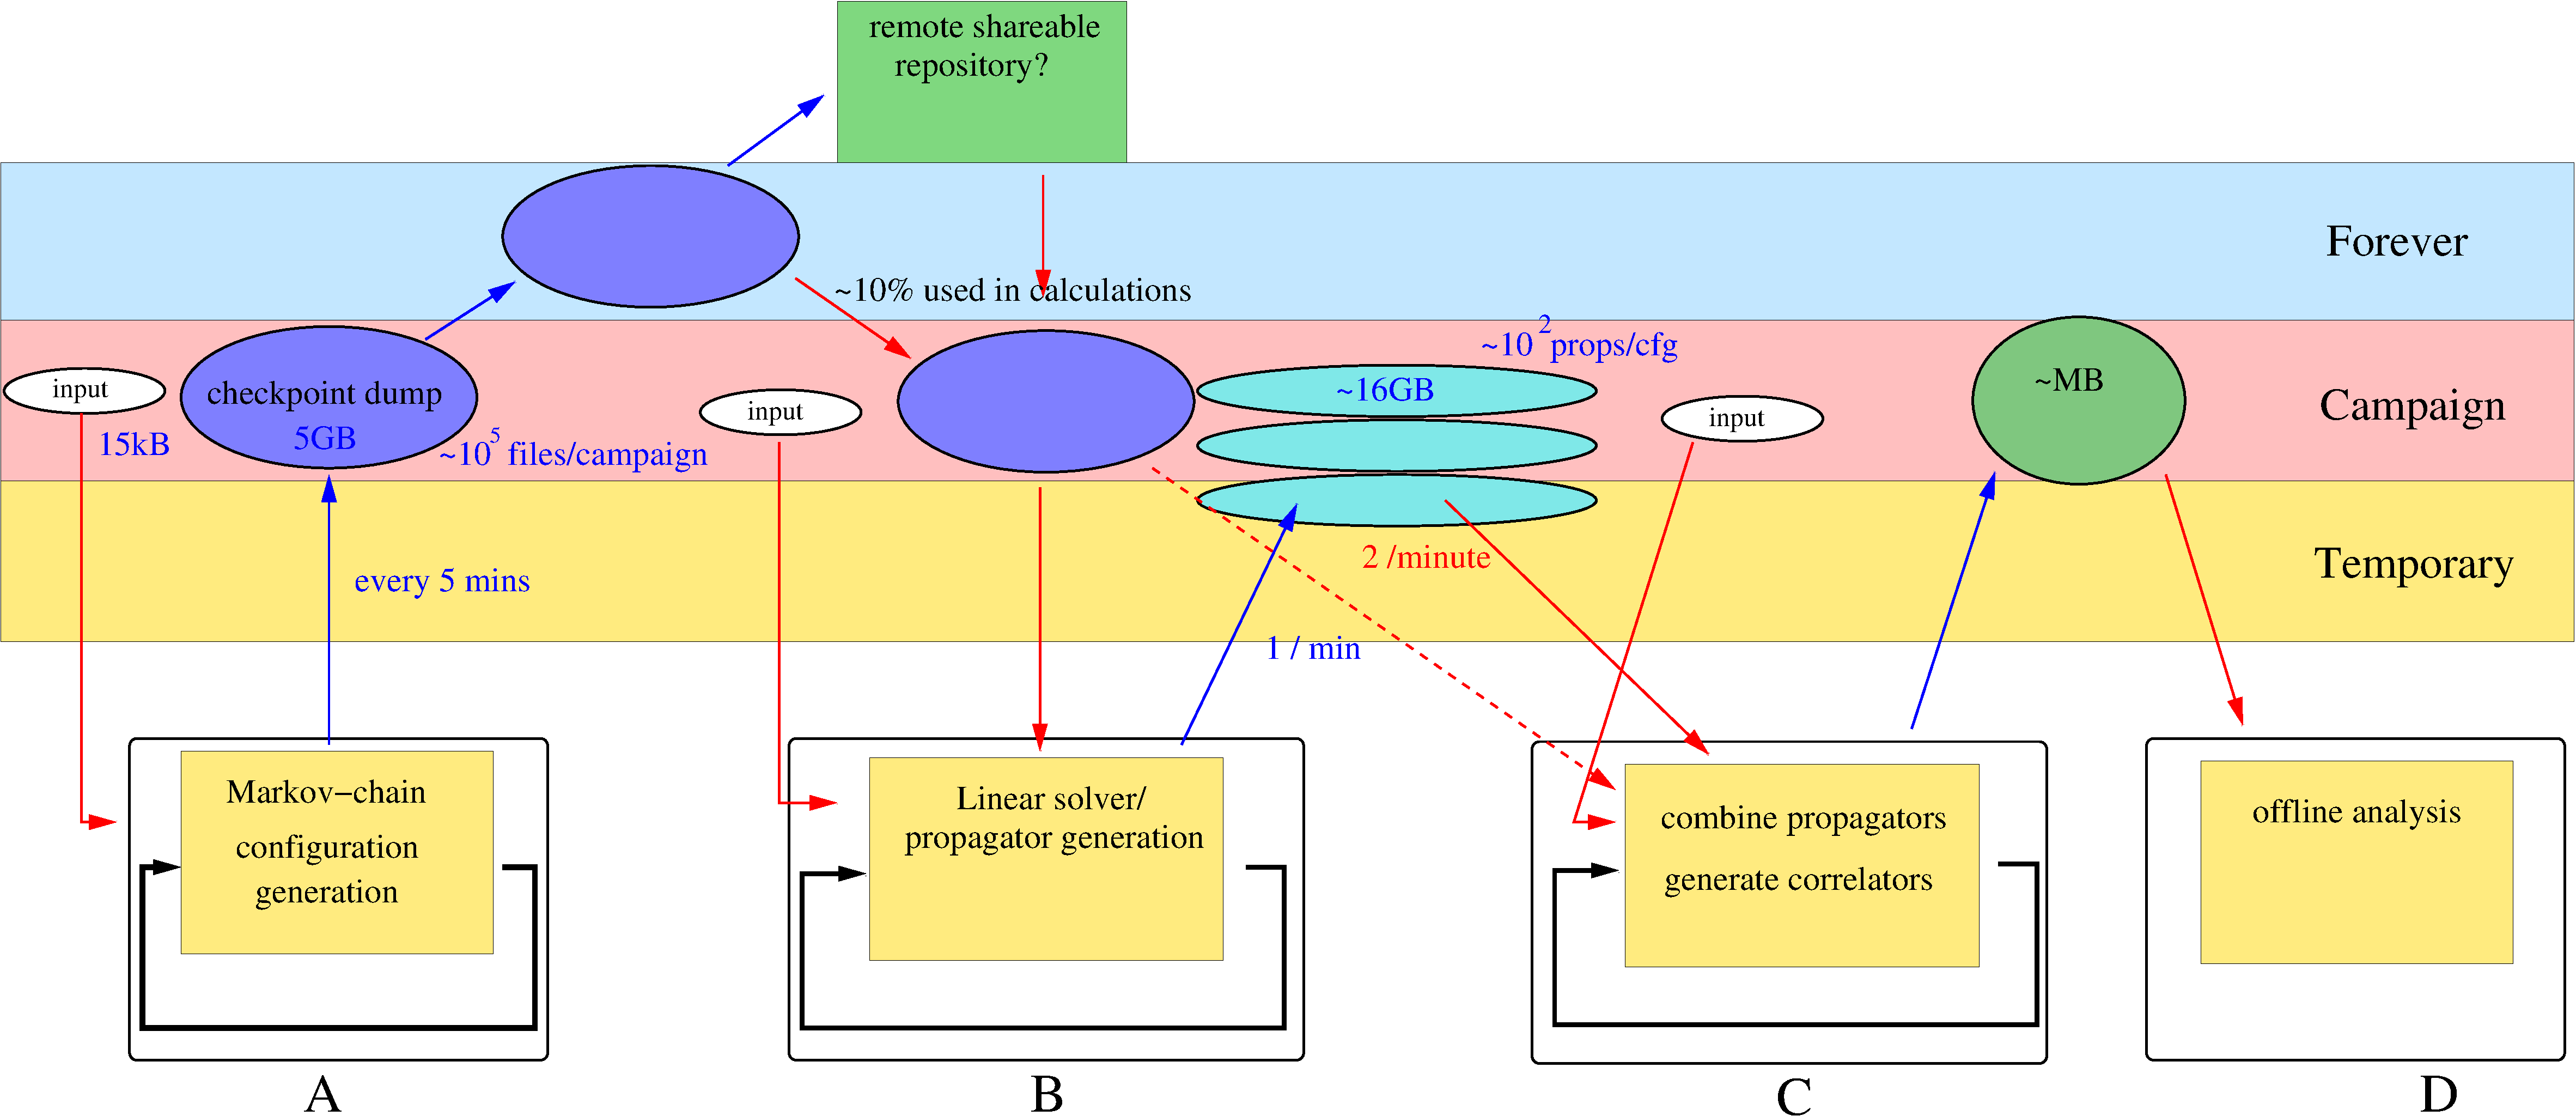
\includegraphics[width=\textwidth]{FIGS/lqcd_workflow.pdf}
    \caption[The LQCD workflow]{ We can put a longer caption in the curly brackets. The short caption in square brackets goes in the List of Figures}
    \label{fig:lqcd_workflow}
\end{figure}


A lot of reference, such as this one~\cite{Edwards:2004sx}, are already in the IO-SEA.bib database file. To make something show up in the glossary just use flag it like I am doing for \Gls{JSC}. Make sure the term is listed in Glossary.tex. \fxnote{ Maybe this chapter needs work.}